% !TEX encoding = UTF-8 Unicode
%!TEX root = thesis.tex
% !TEX spellcheck = en-US
%%=========================================
\chapter{Project management}
\label{chapterProjectManagement}
\label{chapterPlanning}

Good planning is essential for a large project to be successful. Decisions like assignment of tasks, sketching of solutions, what tools to use, and when and where to meet has to be decided. An organised plan ensures everybody is on the same page and shares a common understanding of what to do.

Planning can be divided into two parts; planning of the system itself (its architecture and technologies), and organisational planning. The organisational plan is mostly decided upon in early project phases, while system planning is done by individual teams along the way, so to ensure common development practices. 

Project management of a microservice project proved to be a new and challenging experience for the team compared to more traditional architectures. Because of the experimental \acrshort{devops}\footnote{DevOps is a movement where the Development and Operations of a system is combined, so that the developers also operate the systems \citep{whatIsDevOps}.} style of the project and microservice oriented product, it was difficult to maintain a traditional Waterfall or Scrum-like development process. Other development processes like the Spiral model were used instead.

\section{Risks}
\label{section:risks}
During the first group meeting the team did a risk analysis to identify and rank the risks' priorities. There were also made contingency plans for each identified risk. The result is displayed in figure \ref{fig:risk_analysis}. A scale from one to nine was used to rate the likelihood and impact of each risk, the importance being given by the product of likelihood and impact. Some risks were added as the project went along, as not all of them were considered initially. 

There were also some adjustments to likelihood and impact. Doing reevaluations of the risk analysis helped give a better understanding and awareness of the risks in the project, which enabled more easily avoiding and handling them. The risk analysis was weekly reconsidered, either by a few of the members, or the whole team depending on availability. The reevaluation was done by taking new experiences and events into consideration when looking at each of the risks and discussing whether there were any risks missing or in need of adjustment.

Initially, the team had one more member, though a few weeks in this member had to leave the project for personal reasons. A member leaving was not one of the risks considered, though the nature of the project architecture mitigated much of the impact by scaling down on the project scope. 

\begin{table}[H]
\begin{center}
\caption{Risk analysis}
\scalebox{0.8}{
\label{fig:risk_analysis}
    \begin{tabular}{ | p{4cm} | l | l | l | p{4cm} | p{4cm} |}
    \hline
    Description & Likelihood & Impact & Importance & Preventive action & Remedial action \\ \hline \hline
    
    Members of the team is absent & 9 & 3 & 27 & Divide tasks and plan ahead, so the remaining members do not lack information to continue working & Contact the absent members to obtain the required information. Redistribute tasks \\ \hline
    Bad/lack of communication & 3 & 5 & 15 & Regular meetings, team building & Team building \\ \hline
    Wrong tools & 3 & 5 & 15 & Do research when new tools are needed and stick to familiar tools & Consider switching to a different tool \\ \hline
    Unplanned absence & 7 & 2 & 14 & Keep everyone updated & Redistribute tasks \\ \hline
    Unrealistic goals & 5 & 2 & 10 & Use techniques such as estimation poker & Attempt to re-estimate and consider working overtime \\ \hline
    Individuals not able to complete task & 5 & 2 & 10 & Inform the group early if you are having trouble & Bring the unfinished tasks to the next sprint, and attempt to finish the task early in the next sprint \\ \hline
    Loss of data & 1 & 6 & 6 & Frequent backups and the use of version control & Recreate data \\ \hline
    Client can not meet & 2 & 3 & 6 & Give the client multiple options on when to meet & Reschedule as soon as possible \\ \hline
    Unclear organisation and responsibilities & 2 & 3 & 6 & Assign clear roles early & Reorganise if possible \\ \hline
    The skill of individuals does not match the given task & 6 & 1 & 6 & Map skill/knowledge early & Internal courses, homework readings \\ \hline
    
    \end{tabular}
}
\end{center}
\end{table}

\section{Absence}
%%
Over the course of a project this scale, it is to expect that some members are absent or busy for periods of time. Mapping out prolonged absence early helped determine available resources each week. This was important in planning how to distribute the workload and when to implement different parts of the system. 
%%
For example, from week 10 to 13 half of the team went on an excursion. During this time no major implementations were being developed, and the absent team members were only assigned minor and documentation related tasks. 

Figure \ref{plannedAbsence} shows the table of when people knew they would be busy. In addition to the written status, the figure was colour coded for easy readability. Each status was defined as follows:
% ^ This should resolve the previous issue with greyscale stuff, as the table legend
% now includes the words and what they mean.
\begin{flushleft}
\begin{itemize}
\itemsep -0.5em
    \item Green : Available, reply within 8 hours.
    \item Yellow : Mostly available, reply within 24 hours.
    \item Bright red : Somewhat busy, will reply when time.
\end{itemize}
\end{flushleft}

\noindent Initially there was also a dark red status, indicating inability to respond until the following week. This was not used, as the team had multiple communication channels and had made arrangements for team members to be at least moderately reachable at all times. More information about the use of communication tools can be found in section \ref{sectionCommunicationTools}.

\begin{figure}[H]
    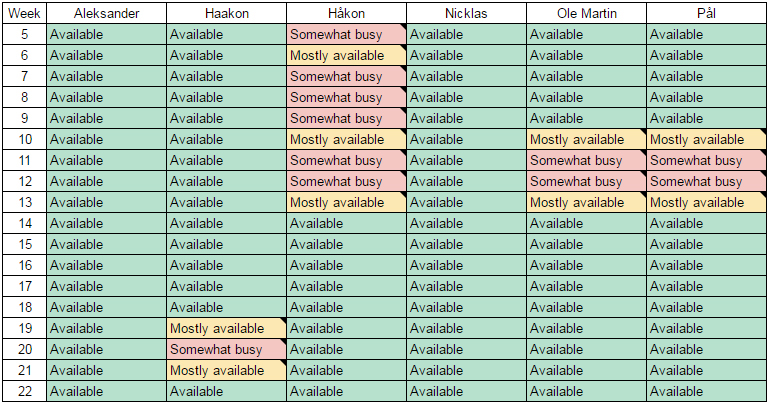
\includegraphics[width=\textwidth]{tables/planning/whereAreYou}
    \caption{Planned absence}
    \label{plannedAbsence}
\end{figure}


\section{Time frame}

\if  %% If False starts here #####################
\todo[inline]{ What to include: (Btw no clue how to structure this. Timeline, table, list, idk?)
\\ {[}Prio: Low{]} }
\begin{itemize}
    \item Feb 12. Preliminary report
    \item Feb 25. VERY early demo. Just thoughts and drawings
    \item March 7. Deadline for content:editor, auth and communication
    \item March 7. First working demo for client
    \item March 18. Midterm report
    \item March 31. Deadline for Search:back-end
    \item April 11. Deadline for Content:publication
    \item April 25. Deadline for Content:datasets and Content:site-administration
    \item May 1. Deadline for deploying the system
    \item May 31. Deadline final report. 
\end{itemize}
\fi   %% If False ends here #######################
Group members were expected to each spend roughly 20 hours per week on the project, as it is a 15 credits course.
This resulted in 120 work hours per week at the teams disposal. This was originally 140 hours, though a group member left the team and course early on. Despite this, it was still planned to have 3 teams each working on different tasks throughout most of the project. For some tasks this partitioning turned out to be too small or too big. In those cases, the relevant teams were adjusted accordingly. 

Figure \ref{fig:deadlines} shows a planned timeline for working on the various tasks. 

The deployment deadline was set to 1st of May. This was decided primarily to leave May for writing the report and documentation. It also left sufficient time in case of underestimated time required for development tasks.

Figure \ref{fig:deadlines} shows when to implement each service and which are being developed in parallel. Lines 1, 4, and 8 represent report deadlines, lines 2, 3, 6, 7, and 9 represent development deadlines and demonstrations of the system, and line 5 represents the Easter holiday. It is due to its span over the Easter that the search service task is as long as it is.

\begin{figure}[H]
    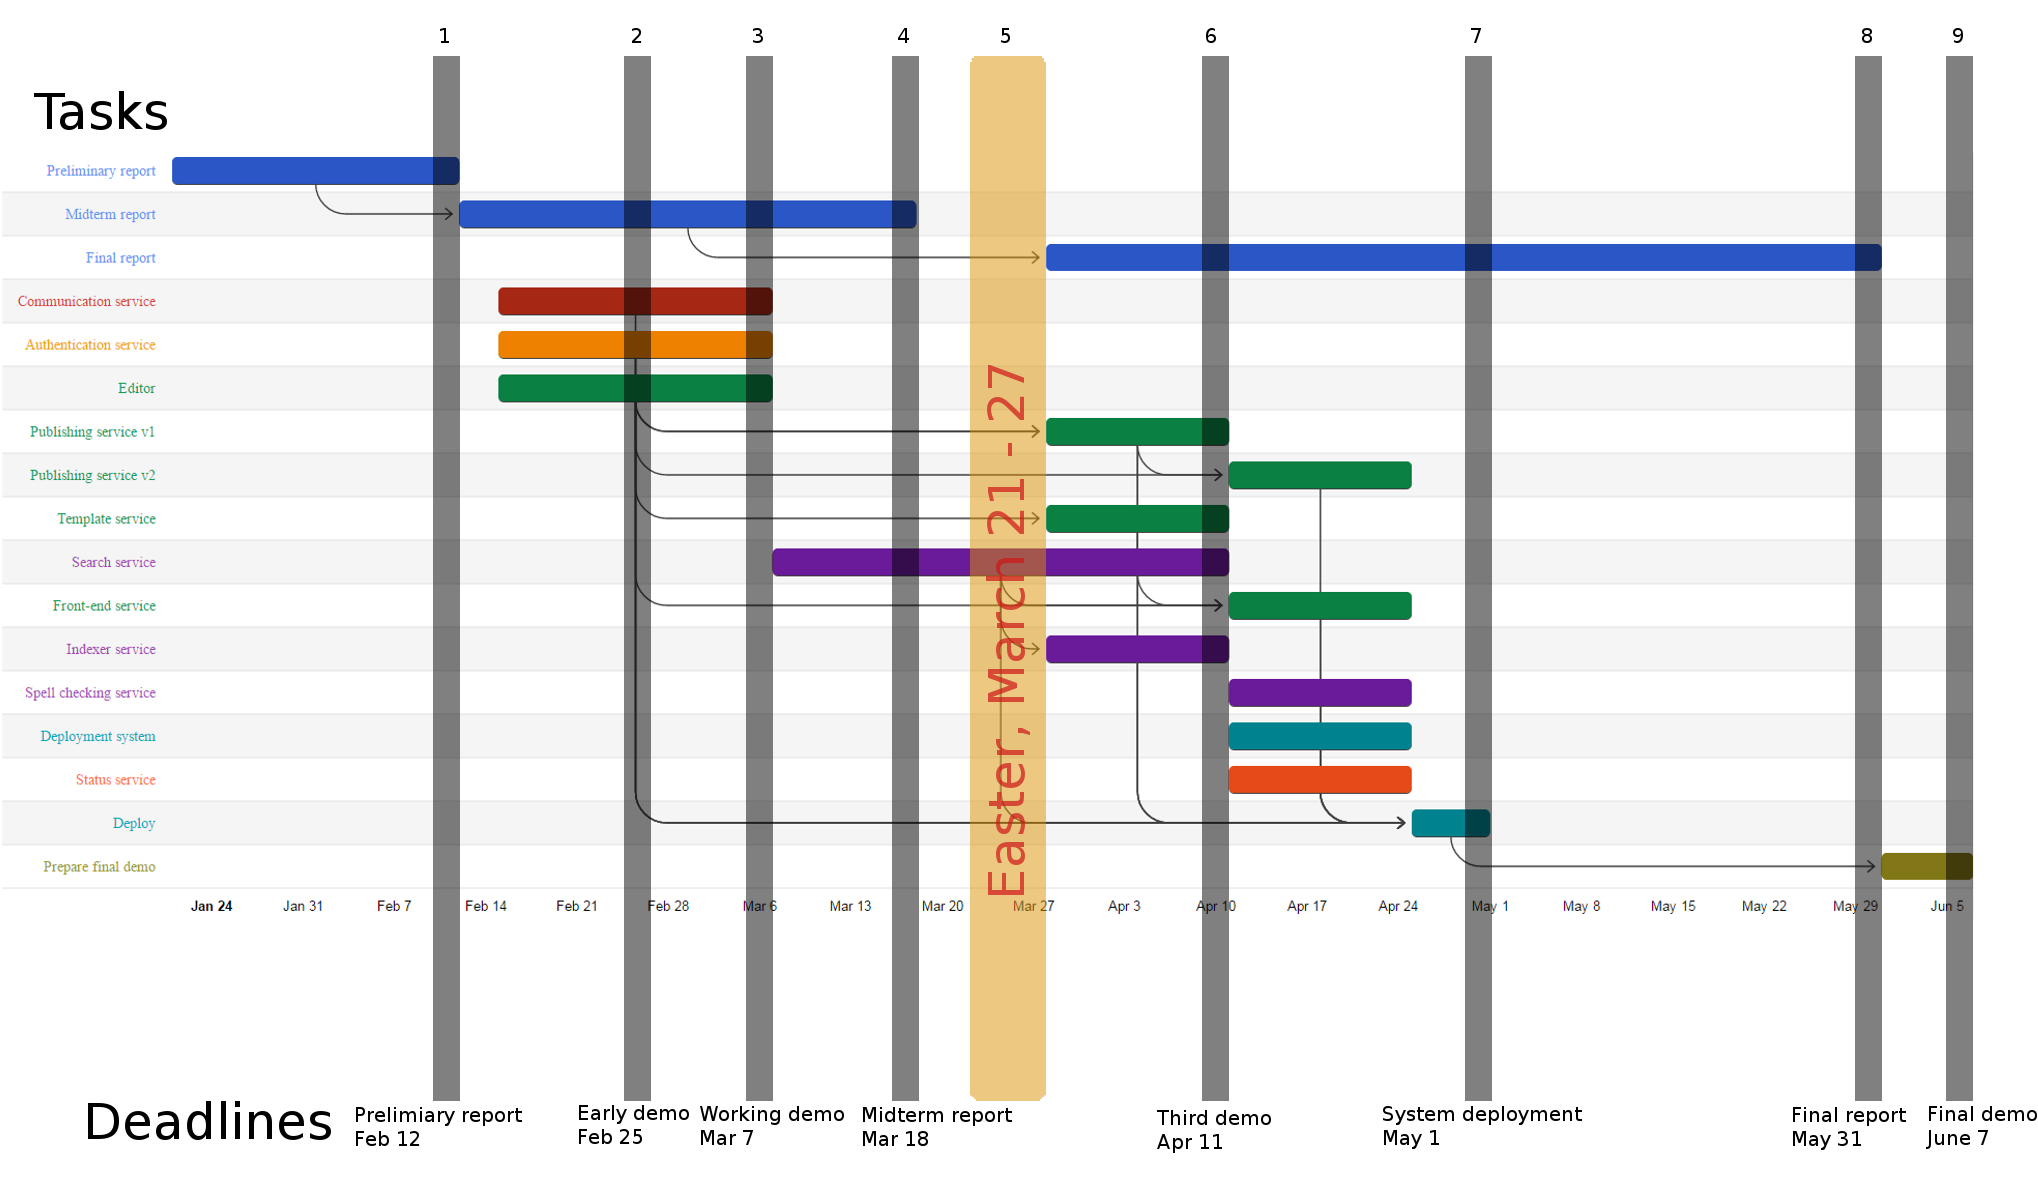
\includegraphics[width=\textwidth]{fig/plan}
    \caption{Activity plan with tasks and deadlines. Arrows indicates dependencies.}
    \label{fig:deadlines}
\end{figure}

\section{Estimation}

With a lot of focus on researching and exploring advantages, problems, and best practices -- estimating each task down to hours was both unpractical and infeasible. Some attempts towards estimating tasks in hours were made early in the project, though was quickly abandoned and story points were to a degree used instead \citep{storyPoints}. This allows for a more abstract estimate, while not committing to a fixed number of hours. In practice, the story points represented days until launch of the service, one day being about eight work hours. This type of measurement better handles all the uncertainties related to the research needed for each service. 

\section{The team}
During the first meeting, all the team members filled out a form with past experiences and language/technology familiarities. This was meant to be an aid for how to pick the members for the sub teams for the different microservices. The results from the meeting are displayed in table \ref{table:theTeam}. 

\begin{table}[H]
    \caption{The team, knowledge mapping}
    \centering
    %\begin{tabular}{| l | p{5cm} | p{5cm} | l }
    \begin{tabular}{|l|p{5cm}|p{5cm}<{\raggedright}|}
    \hline
    \textbf{Name} & 
    \textbf{Languages/technologies} & 
    \textbf{Experiences} 
    \\ \hline
    
    Aleksander Hansen & 
    Python, Java, C\#, C++, HTML, JS, LaTeX, MySQL, git & 
    IT1901
    \\ \hline
     
    Haakon Johansen Jonsson &
    Python, C/C++, Java, Scala, LaTex,  MySQL, Android, git & 
    Misc. small android projects, IT1901 
    \\ \hline
    
    Håkon Larsen Solbjørg & 
    Python {[Django]}, git, Java, HTML, JS, CSS, REST, LaTeX, UNIX, CI, Testing &
    dotkom, the startup Islero, IT1901
    \\ \hline
    
    Nicklas Nilsen & 
    Python, SQL, Fortran, LaTeX, git, UNIX & 
    IT1901 
    \\ \hline
    
    Ole Martin Knurvik & 
    Python, CSS, HTML, JS, Java {[Android]}, LaTeX, C\#, git & 
    Design and \acrshort{ui}, IT1901
    \\ \hline
    
    Pål Karlsrud & 
    Python {[Django, Flask]}, Java, C, Perl, Postgres, MySQL, UNIX, Apache, Shell, git, HTML, JS, CSS & 
    IT-Komiteen at Samfundet, IT1901
    \\ \hline
    \end{tabular}
    \label{table:theTeam}
\end{table}

\section{Team organisation}

The internal teams were assigned and reassigned based on the current requirements and technologies used, so having strictly defined roles throughout the project would have been cumbersome. Although some overarching responsibilities were assigned to some team members, to ease communications and knowing who to talk to regarding e.g.\ service hosting and operations during testing.

\subsection{Roles}
  
\paragraph{Group Leader} Ole Martin Knurvik\newline
The group leader took care of organisational tasks and delegated work to the other group members. Examples of tasks are booking meeting rooms, communicating with the customer and course staff, et cetera.
  
\paragraph{CTO} Håkon Larsen Solbjørg\newline
The \acrlong{cto} is a role which functions as an advisor. This can be useful when starting developing a feature, for example suggesting a programming language, framework, or library to use, or a sparring partner on how to implement a given functionality.


\subsection{Responsibilities}

\paragraph{UI and UX} Ole Martin Knurvik\newline
Has the executive role of design (\acrshort{ui} and \acrshort{ux}) for the front-end service(s) of the system. This covers following a graphic profile, making sure the design is clean, and that the system is usable from a usability perspective. This role originally included responsibility for usability testing and such, but was omitted seeing as this is not important for an architecture demonstration.

\paragraph{Deployment server(s) (production)} Pål Karlsrud\newline
Has the executive responsibility of managing the deployment server(s) that are used in a production environment.

% hihi, tusen takk! :D
% Ikke enda dessverre :p Drar dit straks! Yaaay! Masse flott lagg! Gleder meg masse. 
% Ohhhh! Det er sweet! Det kan egentlig hjelpe ganske mye :D

% HEI PÅL :D
% \paragraph{Gratulerer med dagen i går!} :D
% Er du på toget? TUUT TUUUUUT
% :(
% :'(((
% Sharelatex på NSB <33 blir sikkert bra. Websockets over treg 3G. 3ge? EHHEHEHEHEHHEH E HEHHEHEEH 
% Vi kan synce sharelatex mot github nå btw

% TakK!
% Vil du være med`?

% Det hadde vært litt dumt å bruke "chat" funksjonen i ShareLatex egentlig
% Det her er jo mye bedre
% Kan se alle typoene til folk underveis :D
% hahahah, en halv kek
%kek
% nice chat
%jeg er på vei nedover. skal prøve å rename sprintene 

% Bra vi hadde denne chatten i mellom to subparagraphs da, og ikke mellom den siste 
% paragrafen og neste section ,_,

% x)

% LA STÅ ^

\paragraph{Staging server(s) (development)} Pål Karlsrud and Håkon Larsen Solbjørg\newline
Has the executive responsibility of managing the staging server(s) that are used in a development environment.


\section{Software development process}
\label{section:devProcess}
The overarching guideline of the project was to explore and demonstrate the microservice architecture, rather than an implementation of the product itself. 
A consequence of this was that Scrum and Kanban would be difficult to strictly follow, as many of the elements from these methodologies would have seemed like wasted work. This includes elements like Scrum's product backlog, and Kanban's \acrshort{wip} limits. Initially Scrum was considered to be used as the main development process, but it was abandoned in the early phases of the project.
With a lot of time dedicated to reading up on microservices, methods, and technologies -- following a spiral model was more natural. 
A spiral model enables using part of the planning phase to do research, and iteratively determine the objectives and what functionality to implement \citep{sprialModel}.

This is not to say no elements from other methodologies were used. Daily stand-up meetings were used to keep everyone up to date on how the others were doing, allowing them to come with suggestions and feedback when needed. The objectives of each iteration could also be compared to the sprint backlog in Scrum, or To Do in Kanban. 


As shown in figure \ref{devMeth}, there are four main phases of each iteration. Each iteration started with research, as gathering knowledge about best practices, advantages, disadvantages, and customer preferences was essential in determining the next set of objectives -- in this case which functionalities to implement -- to best demonstrate microservices.

In step two of the iteration, determining the objectives, the client was often included and encouraged to come with feedback based on ideas and thoughts derived from the research. Once the objectives were established, the risks needed to be mapped out and resolved. In the fourth and final step, development and testing, the objectives were naturally implemented and tested before deployment. Due to the small size of each service this was either done alone or with a partner. In this part, techniques like pair programming or Kanban were options for use. This decision was left up to each team depending on what they felt more comfortable with. 


\begin{figure}[H]
    \centering
     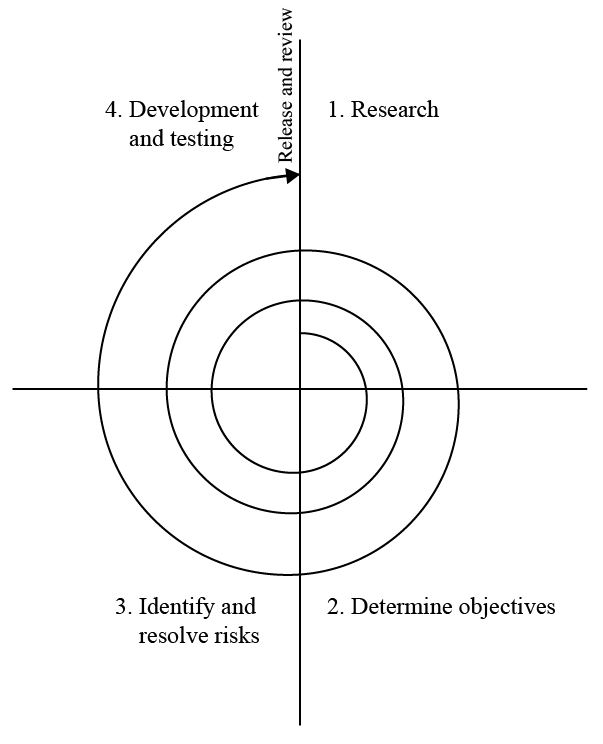
\includegraphics[scale=0.6]{fig/project_management/devMeth}
    \caption{Development method}
    \label{devMeth}
\end{figure}


\section{Iterations}
The length of each iteration has been a bit fluid and varied from one to three weeks. This due to the huge differences in size and uncertainty of each service implementation. Seeing as the team was split into groups which did not depend on each other, apart from the deadlines and deliveries, there was no reason why each group should be locked to the same length for each iteration. 

\subsection{Iteration 1}
\textbf{21st of February -- 7th of March} \\
\noindent During the first iteration, the focus was on three parts of the system: the editor, the authentication service, and the communication service.

The group was divided as follows:

\begin{flushleft}
\textbf{Editor}
\begin{itemize}
\itemsep -0.5em
  \item Haakon Johansen Jonsson
  \item Ole Martin Knurvik
\end{itemize}

\textbf{Authentication}
\begin{itemize}
\itemsep -0.5em
  \item Håkon Larsen Solbjørg
  \item Nicklas Grimstad Nilsen
\end{itemize}


\textbf{Communication}
\begin{itemize}
\itemsep -0.5em
  \item Pål Karlsrud
  \item Aleksander Hansen
\end{itemize}

\end{flushleft}

The goal of the iteration was to get a working prototype up and running for a demonstration with the customer the 7th of March.
This prototype was to consist of an editor, which was to communicate with the authentication service. This meant that a user should be able to log in and then use the editor. The user stories that cover this functionality is shown in table \ref{tab:iter1_stories}.

\begin{table}[H]
   \caption{User stories for iteration 1 }
   \centering
   \label{tab:iter1_stories}
   \begin{tabular}{|p{1.3cm}|p{6cm}|p{3cm}|p{2.5cm}|}\hline%
        ID & Description & Service & Story points\\\hline\hline
        
        CF-1 & As a user, I should be able to create articles using a \acrshort{wysiwyg} editor & Front-end & 8 \\ \hline
        CF-2 & As a user, I should be able to add and adjust images & Front-end & 3 \\ \hline
        CF-3 & As a user, I should be able to add videos to articles & Front-end & 3 \\ \hline
        CF-4 & As a user, I should be able to add links to other articles and to web pages & Front-end & 2 \\ \hline
		A-1 & As a user, I want to be able to log in & Auth & 8 \\ \hline
        A-4 & The system should allow for different access levels & Auth & 8 \\ \hline
        COM-1 & The services should be able to communicate with each other & Communication & 13 \\ \hline
        COM-2 & The services should be able to easily query for the \acrshort{ip} address of a given service & Communication & 3 \\ \hline
    \end{tabular}
\end{table}

Most of the iteration was spent on learning and choosing which technologies to use for the various services. This took a lot more time than originally anticipated, as the team had little experience with most of the technologies that were planned for use. This motivated the switch from Scrum to the spiral model.

Combining the services proved to be harder than expected.
While all the services worked by themselves at the end of the iteration, communication between the editor and the authentication service was not ready for the demonstration.

During the course of the iteration it was decided, in agreement with the customer, that a distributed communication system would be used. A \acrshort{wysiwyg}-type editor was chosen, and templates were to be fully editable. ``Embedded code'' was interpreted to mean embedded objects like video.
The requirements as they were before any changes were made is found in appendix \ref{requirements}.

\subsection{Iteration 2}
\textbf{28th of March -- 11th of April} \\
\noindent Between the 7th and 28th of March, only the search service was in development; the next proper iteration did not start before the 28th of March. This was due to Easter, having to write on the report, and a large part of the group being unavailable.

The second iteration focused on the first publishing service, the template service, the search service, and the index service.

The group was divided as follows:

\begin{flushleft}
\textbf{Publishing service}
\begin{itemize}
\itemsep -0.5em
  \item Haakon Johansen Jonsson
  \item Ole Martin Knurvik
\end{itemize}

\textbf{Template service}
\begin{itemize}
\itemsep -0.5em
  \item Pål Karlsrud
  \item Håkon Larsen Solbjørg
\end{itemize}


\textbf{search and indexer service}
\begin{itemize}
\itemsep -0.5em
  \item Nicklas Grimstad Nilsen
  \item Aleksander Hansen
\end{itemize}

\end{flushleft}

The goal of this iteration was to create an improved prototype, capable of demonstrating publishing and viewing of articles, searching, and loading templates. The user stories that cover the functionality in this iteration is shown in table \ref{tab:iter2_stories}.

\begin{table}[H]
   \caption{User stories for iteration 2 }
   \centering
   \label{tab:iter2_stories}
   \begin{tabular}{|p{1.3cm}|p{6cm}|p{3cm}|p{2.5cm}|}\hline%
        ID & Description & Service & Story points\\\hline\hline
        
        CF-5 & As a user, I should be able to view articles in an appropriate \acrshort{ui} & Front-end & 3 \\ \hline
        CT-1 & As a user, I should be able to choose a template for the article & Template & 13 \\ \hline
        CP-1 & As a user, I should be able to publish created articles & Publishing & 8 \\ \hline
        CP-2 & As a user, I should be able to edit metadata (tags and descriptions) of documents & Publishing & 2 \\ \hline
        SE-1 & As a user, I should be able to quickly search for documents & Search & 13 \\ \hline
    \end{tabular}
\end{table}

The improved prototype did have the features that were planned to be implemented in this iteration. The template and search services were not connected to the front-end, and had to be demonstrated by themselves. The publishing service however could demonstrate communication between services.

The original plan was to have every microservice supply their own user interface, and have the client-side load them individually
During the iteration it was decided that there would be a separate front-end service to deal with the user interface, because communication within the client-side of the project turned out to be really difficult. After the demonstration for the customer, an additional requirement -- having two implementations of the publishing service -- was added by request from the customer. It was also decided that features like calendar information, attachments, and support for different file types in the search service, were not important to the goal of the project, so the related requirements were removed.